\documentclass{article} %DO NOT CHANGE THIS
% for the title offset
\usepackage{titling} 
% for images
\usepackage{graphicx} 
% for page margin
\usepackage[margin=0.8in]{geometry} 
% for math expression
\usepackage{amsmath}
\usepackage{nccmath}
% for formatting
\usepackage{multicol}
\usepackage[super]{nth}
% for specifying captions to tables and figures
\usepackage[font=small,labelfont=bf]{caption}
\author{
  Goh Wei Wen\\ \\
  \texttt{A0156085B}
  \and
  Kevin Leonardo \\Anantha\\
  \texttt{A0161302Y}
 \and
  Li Hong Sheng \\Gabriel\\
  \texttt{A0104274N}
  \and
  Li Jiayao\\ \\
  \texttt{A0160257J}
  \and
  Zhang Shuoyang\\ \\
  \texttt{A0158000X}
}
\title{Learning to Play Tetris with Big Data}
\begin{document}
\maketitle
% * <goweiwen@gmail.com> 2018-04-20T06:00:43.520Z:
% 
% I think we should restructure to fit a normal research paper format:
% Abstract (explain new knowledge and results briefly)
% Introduction (explain the problem)
% Methodology (details of GA, expectimax)
% Results (weights trained, performance)
% Discussion (how to improve, other attempts)
% Related works (maybe optional for this, but it should contain other related work in this area)
% Conclusion
% 
% ^.
\begin{abstract}
\noindent
\textsl{Tetris} is a popular computer game. The player is given a sequenece of randomized tetromino pieces one at a time and must pack them into a rectangular gameboard. Any completely filled row of the gameboard is cleared and all filled squares above it are shifted down by one row. We have designed an utility-based agent to play \textsl{Tetris} which is able to clear millions of rows by maximizing the number of rows cleared. We illustrate how the agent is able to achieve this with the help of \textsl{genetic algorithm}, and our game playing strategy, \textsl{expetimax},  which is used in optimally positioning a randomly given tetromino. Besides, we describe the method utilised to enable our agent to scale up to big data. Furthermore, we showcase the performance of the learning algorithm and its speedup on big data. Last but not least, we discuss the areas that we can further improve on to obtain a better result. 

%combine GA and expectimax as the result is achieved by both of them.
% which learns an optimal values for a set of pre-determined criteria, called features - they enable the agent to evaluate the optimality of a move.

%we use "game playing strategy" all the way

\end{abstract}
\begin{multicols}{2}
\section{Introduction} \label{intro}
\textsl{Tetris} is a popular computer game invented by mathematician Alexey Pazhitnov in the mid-1980s \cite{Tetris}. The goal of the game is to clear as many rows as possible. In this paper, we present a \textsl{genetic algorithm} that learns a set of weights for an utility function, combined with expectimax, which attempts to optimally position (by rotating 90$^\circ$ or 180$^\circ$ in any direction ) a piece of tetromino on a \textsl{Tetris} grid. The learning process of this algorithm is detailed in section \ref{learning-method} and game playing strategy in \ref{Game-play Strategy}. Empirical results, in section \ref{results}, show that our algorithm is able to learn a set of weights to play Tetris within a relatively short period of time, and it scales relatively well when run on big data.\\ \\
\noindent
The gameboard we used in the project is a $10$ rows $\times$ $20$ columns 2D grid. The 7 pieces of tetromino used in the game are shown below:

\begin{center}
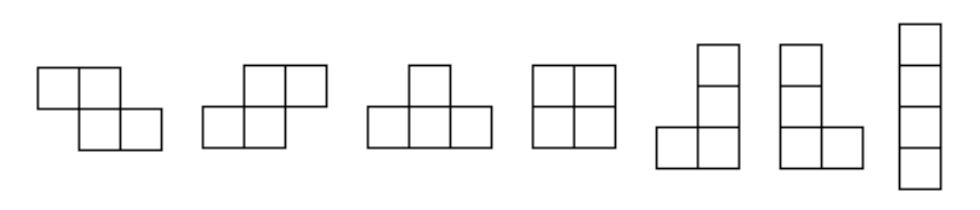
\includegraphics[width=8cm,height=10cm,keepaspectratio]{tetris_shapes.JPG}
\end{center}

\noindent
The game begins with a blank grid and ends when the last shape that is placed reaches the top of the grid. The \textbf{goal} of this game is to \textbf{maximize} the number of rows cleared.

\section{Methodology}
\subsection{Features} \label{features}
% specify the features are used in GA
The following 6 features that are used in our \textsl{genetic algorithm} were taken from an article\cite{citefeatures} with some modifications.
\begin{enumerate}
  \item \textbf{Height difference}: the height difference between the highest colnum and the lowest colnum in the gamboard.
  \item \textbf{Number of rows cleared}: number of rows whose cells have been completely filled (and thus removed from the grid).
  \item \textbf{Row Transitions}: a row transition refers to the occurrence of a filled cell next to a hole in the same row.
  \item \textbf{Column Transitions}: a column transition refers to the occurrence of a filled cell that is next to a hole in the same column.
  \item \textbf{Number of Holes}: number of empty cells in the grid such that each cell has at least one filled cell on top of it in the same column.
  \item \textbf{Number of Wells}: wells refer to groups of holes whose left and right cells have been completely filled.
\end{enumerate}
Each of these features is assigned a \textbf{real-valued} weight, which is used by our utility function to estimate the optimality of a state. Let S be a state, $w_n$ be the weight for the nth feature $t_n$, the utility of S can be represented by the following function:

\begin{ceqn}
\begin{align} \label{eq:1}
f(S) = \sum _{n=1}^{6} w_n \times t_n
\end{align}
\end{ceqn}

As mentioned in equation \ref{intro}, we aim to maximize $f(S)$ for each random given tetromino piece.

% A move that leads to a state with more features with high-valued weights is more likely to be chosen over another that has more features with low-valued weights during game-play as described in section \ref{Game-play Strategy}.

% * <goweiwen@gmail.com> 2018-04-20T05:52:24.328Z:
% 
% This is our current list of features: https://github.com/JYL123/CS3243-Project/blob/bc06099de4ce8ec1dd3347075a24c78959404c58/PlayerSkeletonSubmission.java#L82
% 
% ^.
% we use "an optimal weight" instead of "the" because there may be mutiple optimal values
\subsection{Learning Method}\label{learning-method}
To maximize the equation \ref{eq:1}, we run our \textsl{genetic algorithm} to learn an optimal weight ($w_n$) for each feature ($t_n$). A high-level description of our genetic algorithm is outlined as below:

\begin{enumerate}
\item \textbf{Initialize population}: a population is a list of individuals. Each individual of the population is a $1 \times n$ weight matrix, where n is the number of features that we have chosen, as listed in \ref{features}. More formally, suppose that we have weights $w_i$, $w_{i+1}$, $w_{i+2}$ ... $w_n$. Then, each individual can be represented as an $n$-tuple:
% * <goweiwen@gmail.com> 2018-04-20T05:48:51.808Z:
% 
% Our population can be simply a set of individuals, since the order does not matter.
% 
% ^.

$$
[ w_1, w_2, ..., w_i, w_{i+1}, w_{i+2}, ..., w_n ]
$$

In our setting, the initial weights are generated randomly. Specifically, for features, height difference, row transitions, column transitions, number of holes and number of wells, the initial weights are a random \textsl{negative} number between 0 to 1. For feature, number of rows cleared, the initial weight is a random \textsl{positive} number between 0 to 5.  

\item \textbf{Evaluate the initial population}: this is achieved by playing \textsl{Tetris} using each set of weights in the population. The evaluation score for each individual is the \textsl{total number of rows cleared} in the game. One point to note is that in order to fairly evaluate each individual, we evaluate each individual 5 times and take the average of these 5 scores as the final score for the individual.

% not here
% After all individuals are done "playing" the game, update the best score and corresponding weight values that were used to obtain that score.

\item \textbf{Tournament selection}: tournament selection is a robust selection mechanism that is commonly used in genetic algorithms \cite{tournamentselection}. In our setting, we utilize binary tournament selection, a simple mechanism to select a better individual among 2 randomly chosen individuals to produce the next generation. Therefore, a parent with a higher score is more likely to be chosen in \textsl{tournament selection}. Suppose the score for individual $ i $ is $ s_i $. The population can now be seen as list of individual scores:

$$
[s_1, s_2, s_3, ..., s_{n-2}, s_{n-1}, s_n]
$$

In our setting, we first randomly choose 2 individuals from the top 50\% of the population. Then, we select the better individual among these two to be a \textsl{parent}. In the same way, we select another individual to make up a pair of \textsl{parents} to produce a child, which is a set of weights. This can be visualized in the partial tournament tree shown below:

\begin{center}
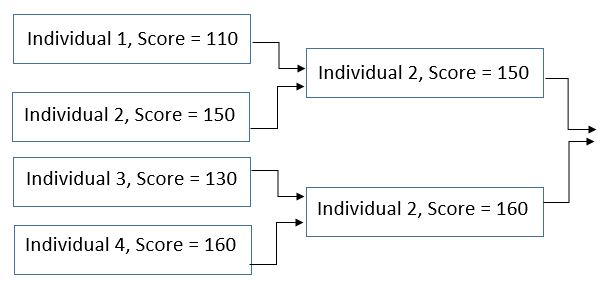
\includegraphics[width=6cm,height=8cm,keepaspectratio]{tournament.JPG}
\end{center}

The child's set of weights is obtained from its 2 parents, with weights randomly selected from each of the parent. By using \textsl{tournament selection}, the next generation is produced.

% we just have to illustrate how tournament selection works, so the explainaiton of size of population is not necessary here.
% The selected individuals of the population (those in the top 50\%) are randomly paired up in the first stage. The best score is from each of the pairs is the "winner" from each stage. Clearly, the tournament selection will select only one "winner". However, we must keep the population size fixed even after tournament selection. Hence, if there are $ N $ selected individuals initially, then we must produce $ N $ "winners" by repeating the tournament selection exactly $ N $ times. Note that there may be some individuals that appear as the "winner" more than once.

% * <goweiwen@gmail.com> 2018-04-20T05:50:01.106Z:
% 
% Maybe explain how tournament selection decreases the chance of a weak individual surviving? by choosing the better of the two.
% 
% ^.

\item \textbf{Swap mutation}: in our setting, a classical mutation method, \textsl{swap mutation}, is utilized in the algorithm. \textsl{Swap mutation} is a simple O(1) operation that is easy to perform with small computation cost compared to other mutation methods, such as insertion, inversion, and displacement which changes all weights in the worst case \cite{swapmutation}. To preserve the optimality of the \textsl{parents}, we will not explore the search space of weights too far away from the current maximum to avoid getting worse weights. Therefore in our setting, the mutation occurs when a probability following \textsl {Gaussian distribution} surpasses a certain threshold set by us. 

% on the new population by randomly swapping weights for different features. E
% * <goweiwen@gmail.com> 2018-04-20T05:50:43.049Z:
% 
% Explain this step more formally as well since there are many different ways to do mutation
% 
% ^.

\item \textbf{Result}: in our setting, we keep track of the highest evaluation score obtained and the corresponding set of weights over 25 generations, with a population size of 25 individuals. 

\end{enumerate}
 

\subsection{Optimized game-play using expectimax}\label{Game-play Strategy}
We used the expectimax algorithm with depth 1 using our utility function as a heuristic for improving how each individual in the population selects the next tetromino piece to play in the \textsl{Tetris} game (i.e. the number of rows cleared would be maximized by that move). \\

\noindent
At each turn, all possible moves (orientations and positions) of the current piece are evaluated using a utility function. The utility function is a weighted sum of different features of the board after a move is played (refer to equation  \ref{eq:1}). The actual weight for each feature is determined using our \textit{genetic algorithm}. \\

\noindent
After a utility function with the most optimal value for each weight is generated, we use the expectimax algorithm to select the next optimal move for each individual of the population. For each legal move, the algorithm looks ahead one piece and calculates the weighted average (using the piece history as weights) of the utility of the board after the best move is selected. Assuming the piece history accurately represents the piece frequency, the algorithm will choose the move with the highest expected utility. \\

\noindent
In contrast to minimax, this strategy does not assume that the adversary will pick the most optimal move. Thus, we cannot prune less-optimal branches, resulting in expectimax being significantly slower than minimax. However, similar to Rodgers and Levin (2014) \cite{expectimax}, we achieved better results when using expectimax over minimax for \textsl{Tetris}. This can be attributed to the fact that we use our additional knowledge of the adversary (the fact that it selects i moves randomly) to our advantage instead of assuming the worst case.

% Reference:
% https://ieeexplore.ieee.org/abstract/document/6932920/
% 
% ^.
% * <goweiwen@gmail.com> 2018-04-20T05:54:49.713Z:
% 
% Also explain that we use frequency of seen pieces to adjust for special sequences
% 
% ^.
\subsection{Parallelism} \label{para}
As we perform \textsl{genetic algorithm} to select an optimal set of weights, each individual set of weights has to be sequentially evaluated by running \textsl{Tetris} to get its evaluation score. This would potentially incur a huge amount of time, if a large size of population and generations are set. Therefore sequential evaluation of individuals will not being able to scale to big data. To speed up the entire evaluation process, we utilize Java 8 \textsl{parallel computing}, which divids a problem into several subproblems, and solve these subproblems in parallel \cite{parallel}. With parallelism, we run our evaluation process for each individual in the population concurrently and efficiently. The comparison of parallel and sequential programming is analysed in section \ref{learning-rate}, Figure 2.



\section{Performance and Statistics} \label{results}
\subsection{Score and Weights}

The maximum score that our genetic algorithm obtained (without using expectimax for selecting moves) was 311143. The following are the weights used to generate this score:

% \begin{enumerate}
%   \item Height difference: -0.553472
%   \item Number of rows cleared: 0.203025
%   \item Row Transitions: -0.274263
%   \item Column Transitions: -0.810374
%   \item Number of Holes: -0.998441
%   \item Number of Wells: -0.274263
% \end{enumerate}

%  -0.5409023035972038, -0.5779452238352727, -0.08382226928735714, -0.7237267127345023, 2.299698319650534, -0.11110083421382877

\begin{center}
\begin{tabular} { |c|c| }
 \hline
 Height Difference &  -0.08382226928735714 \\
 \hline
 Number of Rows Cleared & 2.299698319650534 \\
 \hline
 Row Transitions & -0.5409023035972038 \\
 \hline
 Column Transitions & -0.5779452238352727 \\
 \hline
 Number of Holes & -0.7237267127345023 \\
 \hline
 Number of Wells & -0.11110083421382877 \\ 
 \hline
\end{tabular}
\end{center}

\noindent
Using these exact set of weights and the expectimax algorithm to select moves during game-play, our algorithm managed to attain a score of approximately \textbf{5 million} within only 9 hours, on a desktop computer with a quad-core Intel Core i7 3.4GHz processor.

\subsection{Rate of Learning}\label{learning-rate}
The display of results seen in \textbf{Figure 1} shows that our algorithm results in well above 100,000 rows cleared, after \nth{10} generation. Moreover, from \nth{15} generation onwards, the algorithm is able to reach above 200,000 in rows cleared, with a high rate of increase.

\begin{center}
\begin{minipage}{1.0\linewidth}
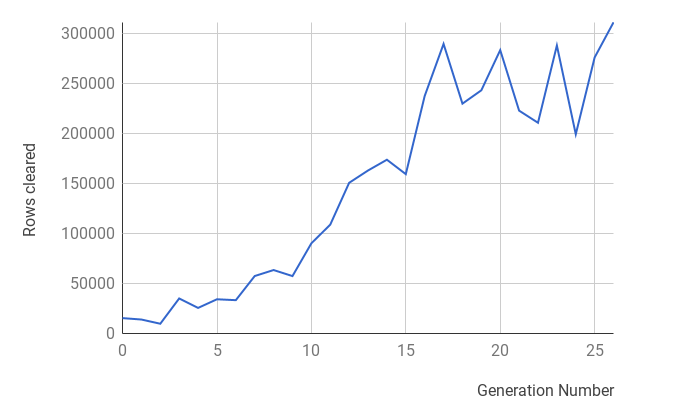
\includegraphics[width=\linewidth]{best_fit.png}
\captionof{figure}{Number of rows cleared for each generation}
\end{minipage}
\end{center}

\noindent
These results indicate that after a few runs of the genetic algorithm, it can play the game quite well. In other words, our algorithm is able to learn a good set of weights within a relatively small number of generations. \\ \\
However, after 20 or more generations, our algorithm is unable to improve its learning on the set of weights, as there is no significant increase in the number of rows cleared. \\ \\
Furthermore, since the AI agent and especially the genetic algorithm have a lot of operations to process, we decided to use parallel processing to speed it up to scale big data (as mentioned in section \ref{para}). \textbf{Figure 2} shows the comparison of time taken between parallel programming and sequential programming for the same generation number. Note that from the \nth{10} generation onwards, the time taken for sequential programming to spawn new generations is too long so we chose not to display it on the graph.

\begin{center}
\begin{minipage}{1.0\linewidth}
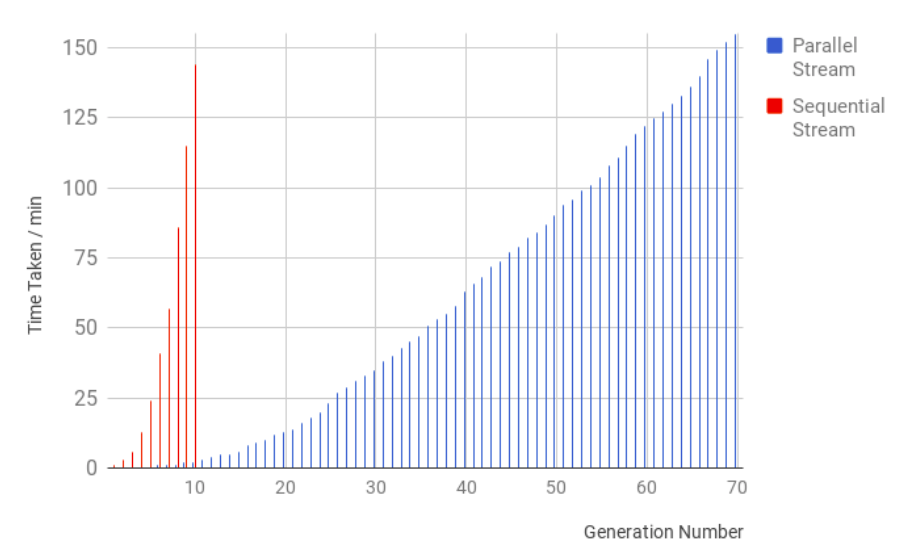
\includegraphics[width=\linewidth]{para_seq.png}
\captionof{figure}{Time Taken for Sequential \& Parallel }
\end{minipage}
\end{center}

\noindent
\\
From the graph, it is clear that parallel programming takes much less time to complete each generation as compared to sequential programming. Hence, parallel programming is able to scale.

\section{Future Improvements}
As the analysis in section \ref{learning-rate} shown, our genetic algorithm can demostrate a good learning rate from \nth{0} to around \nth{16} generation. Afterwards, the learning rate fluctuates. We may assume that at this point, the exploration of weights conducted by our algorithm in the seach space reaches a local optimal.  Therefore more exploitation of the search space of weights is needed. Considering \textsl{genetic algorithm} might not be the best method of learning the optimal value for the weights. We tested on \textsl{particle swarm optimization} (PSO), a population based stochastic optimization technique \cite{PSO}. However, in our experiment, the number of rows cleared with PSO is not ideal, with an average of 5,000. Therefore, a further research on how to improve the learning rate after reaching a local optimal should be conducted. \\
\\
%This part needs a citation to prove the claim.  
\noindent
Furthermore, our research on the Internet turned up a lot of articles on AI \textit{Tetris} agents that used different sets of features with varying degrees of success. Perhaps, we could have experimented with a larger variation of those features. This might help our genetic algorithm to learn a reasonably optimal set of weight values even faster.

\section{Conclusion}
The \textsl{genetic algorithm} presented in this report has been used to learn a set of metrics/weights that is used to maximise the utility output by our utility function. This utility is an estimation of how good a state would be. By comparing the utility scores, \textsl{expectimax} is able to determine the optimal move (position and orientation) for a random given tetromino piece. Furthermore, using these set of weights, the expectimax algorithm, used for game playing, has been shown to be able to handle at least 5 million tetris shapes (possibly more given more computing power and time). Additionally, parallel programming scales in the learning of weights.

% this is explained by the words in ().
%Do note, however, that this not the absolute maximum score that the algorithm can achieve as the program had to be terminated due to time-constraint.


\end{multicols}
% This  to cl determine make a move that is more likely to yield a better score in the Tetris game (i.e. more number of rows cleared).

\begin{thebibliography}{9}
\bibitem{Tetris} About Tetris. (n.d.). Retrieved from https://tetris.com/about-us

\bibitem{citefeatures}
Kamel, M. A. (2011, June 1). El-Tetris - An Improvement on Pierre Dellacherie’s Algorithm. \textit{imake}. Retrieved from http://imake.ninja/el-tetris-an-improvement-on-pierre-dellacheries-algorithm/

\bibitem{expectimax}
Rodgers, P., \& Levin, J. (2014). An investigation into 2048 AI strategies. \textit{IEEE Digital Library}. Retrieved from https://ieeexplore.ieee.org/abstract/document/6932920/

\bibitem{tournamentselection}
Miller, B. L., \& Goldberg, D. E. (1995). Genetic algorithms, tournament selection, and the effects of noise. 
\textit{Complex systems, 9(3), 193-212}. Retrieved from https://pdfs.semanticscholar.org/df6e/e94e2cf14c38e9cff4d2446a50db0aedd4ca.pdf

\bibitem{swapmutation}
Liu, C., \& Kroll, A. (2016). On the performance of different mutation operators of a subpopulation-based genetic algorithm for multi-robot task allocation problems. 
\textit{arXiv preprint arXiv:1606.00601}. Retrieved from https://arxiv.org/abs/1606.00601

\bibitem{parallel}
The Java™ Tutorials. Retrieved from https://docs.oracle.com/javase/tutorial/collections/streams/parallelism.html

\bibitem{PSO}
Shi, Y., \& Eberhart, R. C. (1999). Empirical study of particle swarm optimization. \textit{IEEE Digital Library}.
Retrieved from https://ieeexplore.ieee.org/abstract/document/785511/
\end{thebibliography}
\end{document}